%%%%%%%%%%%%%%%%%%%%%%%%%%%%%%%%%%%%%%%%%%%%%%%%%%%%%%%%%%%%%%%%%%%%%%%%%%%%%%%%
% Template for USENIX papers.
%
% History:
%
% - TEMPLATE for Usenix papers, specifically to meet requirements of
%   USENIX '05. originally a template for producing IEEE-format
%   articles using LaTeX. written by Matthew Ward, CS Department,
%   Worcester Polytechnic Institute. adapted by David Beazley for his
%   excellent SWIG paper in Proceedings, Tcl 96. turned into a
%   smartass generic template by De Clarke, with thanks to both the
%   above pioneers. Use at your own risk. Complaints to /dev/null.
%   Make it two column with no page numbering, default is 10 point.
%
% - Munged by Fred Douglis <douglis@research.att.com> 10/97 to
%   separate the .sty file from the LaTeX source template, so that
%   people can more easily include the .sty file into an existing
%   document. Also changed to more closely follow the style guidelines
%   as represented by the Word sample file.
%
% - Note that since 2010, USENIX does not require endnotes. If you
%   want foot of page notes, don't include the endnotes package in the
%   usepackage command, below.
% - This version uses the latex2e styles, not the very ancient 2.09
%   stuff.
%
% - Updated July 2018: Text block size changed from 6.5" to 7"
%
% - Updated Dec 2018 for ATC'19:
%
%   * Revised text to pass HotCRP's auto-formatting check, with
%     hotcrp.settings.submission_form.body_font_size=10pt, and
%     hotcrp.settings.submission_form.line_height=12pt
%
%   * Switched from \endnote-s to \footnote-s to match Usenix's policy.
%
%   * \section* => \begin{abstract} ... \end{abstract}
%
%   * Make template self-contained in terms of bibtex entires, to allow
%     this file to be compiled. (And changing refs style to 'plain'.)
%
%   * Make template self-contained in terms of figures, to
%     allow this file to be compiled. 
%
%   * Added packages for hyperref, embedding fonts, and improving
%     appearance.
%   
%   * Removed outdated text.
%
%%%%%%%%%%%%%%%%%%%%%%%%%%%%%%%%%%%%%%%%%%%%%%%%%%%%%%%%%%%%%%%%%%%%%%%%%%%%%%%%

\documentclass[letterpaper,twocolumn,10pt]{article}
\usepackage{usenix-2020-09}

% to be able to draw some self-contained figs
\usepackage{tikz}
\usepackage{amsmath}
\usepackage{makecell}

\renewcommand\theadfont{\bfseries}

% inlined bib file
\usepackage{filecontents}

%-------------------------------------------------------------------------------
\begin{filecontents}{\jobname.bib}
%-------------------------------------------------------------------------------
@Book{arpachiDusseau18:osbook,
  author =       {Arpaci-Dusseau, Remzi H. and Arpaci-Dusseau Andrea C.},
  title =        {Operating Systems: Three Easy Pieces},
  publisher =    {Arpaci-Dusseau Books, LLC},
  year =         2015,
  edition =      {1.00},
  note =         {\url{http://pages.cs.wisc.edu/~remzi/OSTEP/}}
}
@InProceedings{waldspurger02,
  author =       {Waldspurger, Carl A.},
  title =        {Memory resource management in {VMware ESX} server},
  booktitle =    {USENIX Symposium on Operating System Design and
                  Implementation (OSDI)},
  year =         2002,
  pages =        {181--194},
  note =         {\url{https://www.usenix.org/legacy/event/osdi02/tech/waldspurger/waldspurger.pdf}}}
\end{filecontents}

%-------------------------------------------------------------------------------
\begin{document}
%-------------------------------------------------------------------------------


% make title bold and 14 pt font (Latex default is non-bold, 16 pt)
\title{\Large \bf Enhancing Quanto:\\Pruning Techniques for Improved Circuit Identity Generation in Quantum Optimization}

%for single author (just remove % characters)
\author{
{\rm Max von Storch}\\
Technische Universität München
\and
{\rm Johannes Schielein}\\
Technische Universität München
% copy the following lines to add more authors
% \and
% {\rm Name}\\
%Name Institution
} % end author

\maketitle

%-------------------------------------------------------------------------------
\begin{abstract}
%-------------------------------------------------------------------------------
This report summarizes Quanto, a quantum circuit optimizer that uses automated circuit identity generation. We propose enhancements to Quanto by focusing on pruning the search space of possible circuits, aiming to improve computational efficiency and scalability, particularly for larger circuits.  
\end{abstract}


%-------------------------------------------------------------------------------
\section{Part A: Paper Summary}
%-------------------------------------------------------------------------------

\subsection{Context and Importance}

Quantum compilers are used to optimize circuits in an effort to reduce execution time, the noise that naturally arises in quantum computations, or both. Generally, the larger the circuit depth, the noisier the computation, leading to more errors in the results. As quantum programs must be executed many times to obtain an accurate picture of their results, reducing the depth of a quantum circuit not only makes a quantum program faster but also reduces the potential for noise and decreases the number of program evaluations required.
\\\\
Existing quantum compilers focus on mapping logical quantum circuits to quantum devices and their native quantum gates. This involves translating source gates to target gates and adapting the circuit to hardware constraints like qubit connectivity. Typically, only simple circuit identities are used during this process, which overlooks the potential for more complex optimizations.
\\\\
Compilers developed by hardware vendors, such as IBM and Google, primarily address the translation and hardware adaptation aspects but focus less on optimizing the logical circuit by finding comprehensive circuit identities. While circuit identities have been manually identified and automatically generated for single-qubit gates by applying a limited number of rules, no current system automatically finds identities for complete gate sets or optimizes quantum circuits based on these identities.

\begin{figure}
  \includegraphics[width=0.7\columnwidth]{assets/quanto_system.png}
  \caption{Quanto system design}
  \label{fig:quanto_system}
\end{figure}
\subsection{Contributions and Methodology}

Quanto automatically generates circuit identities for full gate sets and operates trough two main phases: (1) Identity generation (2) circuit optimization (Fig. \ref{fig:quanto_system}).

\subsubsection{Circuit Identity Generator}
\textbf{Step 1: Represent the quantum circuit as a grid.}
The algorithm starts by representing a quantum circuit as a grid with a depth $d$ and number of qubits $n$. If no gate is present at a particular position, the identity gate is placed there (Fig. \ref{fig:example_1}).
\\\\
\textbf{Step 2: Generation of all possible circuits for $d = 1$.}
If the gate set contains two-qubit gates, these gates are split into the qubits they operate on ($CX$ gate is split into $CXC$ and $CXT$ as in Fig. \ref{fig:example_1}).
\\\\
\textbf{Step 3: Generation of all possible circuits for $d > 1$.}
All subsequent circuits are generated by iteratively appending circuits of depth one ($d=1$) to each previously generated circuit. This process effectively generates the "cross-product" of circuits with the current depth and circuits of depth one.
\\\\
\begin{figure}
  \includegraphics[width=0.8\columnwidth]{assets/grid_example_2.png}
  \caption{Example grid with identity gate substitution}
  \label{fig:example_1}
\end{figure}
\textbf{Step 4: Calculation of unitary matrices and hash values.}
For each generated circuit, the algorithm calculates the unitary matrix. To avoid expensive computations repeatedly, it computes a hash value (fingerprint) for each circuit based on its unitary matrix.
\\\\
\textbf{Step 6: Create fingerprint database.}
The fingerprints are stored in a hash table, with the circuit structure as the key and the fingerprint as the value (Table \ref{tab:databases}). This enables quick look-up of a circuit’s fingerprint during the optimization phase without recalculating the unitary matrix.

\begin{table}[h!]
  \begin{minipage}{0.4\linewidth}
    \centering
    {\renewcommand{\arraystretch}{1}%
    \begin{tabular}{|c | c|}
      \hline
      \thead{Key} & \thead{Value} \\
      \hline
      $[[H, X], [X, X]]$ & $x7ff\ldots$ \\
      \hline
    \end{tabular}}
  \end{minipage}\hfill
  \begin{minipage}{0.7\linewidth}
    \centering
    {\renewcommand{\arraystretch}{1}%
    \begin{tabular}{ |c | c | }
      \hline
      \thead{Key} & \thead{Value} \\
      \hline
       $x7ff…$ & \makecell{$[[X, X], [X, X]]$ \\
      $[[H, H], [H, H]]$}
      \\
      \hline
      \end{tabular}}
  \end{minipage}
  \caption{\label{tab:databases} Left: fingerprint DB. Right: identity DB}
\end{table}


\textbf{Step 7: Create identity database.}
Circuits with identical fingerprints are stored together, forming equivalence classes of circuits (Table \ref{tab:databases}). Each entry in this hash table represents a set of circuits that perform the same quantum operation.

\subsubsection{Circuit Optimizer}
\textbf{Step 1: Generate tiles.}
The circuit is divided into sub-circuits, referred to as tiles. Tiles have uniform dimensions, with the tile width $j$ representing the maximum depth $d$ of the circuit identities, and the tile length $i$ representing the maximum number of qubits $n$ (blue boxes in Fig. \ref{fig:quanto_tile}). The number of possible $i \times j$ tiles for an $n \times d$ circuit is $(n-i+1) \cdot (d-j+1)$.
\\\\
\textbf{Step 2: Check tile validity.}
A tile is invalid and therefore discarded if it contains a two-qubit gate that is not placed at the boundaries of the tile and is cut off by the tile.
\\\\
\begin{figure}
  \includegraphics[width=1\columnwidth]{assets/quanto_tile2.png}
  \caption{Tile with $i=2$ and $j=3$}
  \label{fig:quanto_tile}
\end{figure}
\textbf{Step 3: Tile lookup.}
If a tile contains a two-qubit gate, that has been cut off only at the boundaries of the tile, the cut off gate has to be replaced by an Identity gate, so that there will be a match in the circuit identity database ( a) in Fig. \ref{fig:quanto_tile}). Now the fingerprint is retrieved from the fingerprint database, without having to calculate the unitary matrix. 
\\\\
\textbf{Step 4: Apply substitution.}
For each tile, the corresponding circuit identities are iterated and evaluated by the customizable cost function (Quanto paper: depth $d$).
\\
\textbf{Step 5: Apply substitution to the circuit.}
The optimizer applies the substitution to the quantum circuit ( b) in Fig. \ref{fig:quanto_tile}). If a $CX$ gate was replaced by an identity gate in the tile, the identity gate in the actual circuit must be replaced by a $CX$ gate during the substitution. 
\\\\
\textbf{Step 6: Repeat process.}
Repeat steps 1-6 for a fixed number of times.

\subsection{Evaluation}
\subsubsection{Generation of novel identities}
Quanto is capable of automatically discovering identities known from previous work and generating novel identities for full gate sets, especially for two-qubit gates. This capability is particularly useful for quantum hardware with non-standard native gate sets.
\subsubsection{Challenge of scalability}
One of the main challenges faced by Quanto is scalability. The space of potential circuit identities scales quickly with $n$ and $d$ as described in the formula below (Symbols in Fig. \ref{tab:scaling}). This is because Quanto generates all possible identites, most of which are suboptimal.

\begin{table}
  \centering
  {\renewcommand{\arraystretch}{1}%
  \begin{tabular}{ | c | l | }
    \hline
    \thead{Symbol} & \thead{Definition} \\
    \hline
    $S$ & total number of possible circuits \\
    \hline
    $S_{l}$ & number of possible circuits per depth \\
    \hline
    $g$ & number of single-qubit gates \\
    \hline
    $t$ & number of two-qubit gates \\
    \hline
  \end{tabular}}
  \caption{\label{tab:scaling}Symbols for scaling formula}
\end{table}

\begin{equation}
     S_{l} =\sum_{r=0}^{\lfloor n/2 \rfloor}\frac{n!}{r! (n-2r)!} g^{n-2r} t^r
\end{equation}

\begin{equation}
    S = S_{l}^{d}
\end{equation}

%-------------------------------------------------------------------------------
\section{Research proposal: Pruning Methods}
%------------------------------------------------------------------------------
\subsection{Motivation}
As stated in the Quanto Paper the number of possible circuits grows exponentially with an increasing number of qubits and
increasing circuit depth. In our opinion this is the biggest limiting factor for this type of optimization since it limits the possibilities to optimize larger circuits.

The original method introduced tiling as a work around while this greatly improves the level of optimization for larger circuits it still doesn't provide the same
quality of optimization and speed as a database of larger circuits would do. 

Another Problem is the size of the database itself. The proposed algorithm in the Quanto paper stores all possible circuit in its database not only the most optimal ones. This adds a lot of redundancy to the database and slows down the optimization stage when looking for minimal identities.\\

Pruning the search space of all possible quantum circuit is in our opinion the most important factor fro improving the optimizer further and therefore worth investigating. 

\subsection{Implications and Limitations}
One important change that comes to the structure of the optimizer is that the dictionary that maps the circuits to its fingerprint cant be created and used any more. This is due to the fact that because of the pruning, the database generator won't iterate over all circuits and can't compute the mapping from circuits to fingerprints any more.

If we would create the dictionary in an additional step we could also group these circuits based on their equivalence with no significant expanse, making pruning basically useless.\\

In our research we limited ourselves to optimizing the depth of the circuit as it was the primary optimization goal of the Quanto optimizer. Further research is required if our approach is also feasible for other cost functions.

\subsection{Notations and Definitions}
Before going over the pruning technique, some words on definitions and important terms that are used in the following sections.\\
We use the same notation for the \textbf{gate set}, \textbf{depth} and \textbf{qubit number} as the Quanto paper does. 

Additionally we define $C$ or $C^1$ as the set of all circuits with $n$ qubits and a depth of one and $C^k$ as all Circuits of length $k$. The $[a]_\sim$ Operator returns all circuits that are equivalent to $a$. We write $a\equiv b$ for $a$ being equivalent to $b$ ($a$ and $b$ have the same unitary matrix).

The cost function is generally denoted with $h(c)$ for a circuit $c$.

\begin{description}
	\item[optimal] A quantum circuit is called optimal if there exists no equivalent circuit (for a specified gate set) with lower cost
	
	\item[Column circuit] A circuit with maximum depth of one
\end{description}

For the concatenation of two circuits $a$ and $b$ with the same number of qubits we write $a\Vert b$. The gates of each circuit get appended \textit{qubit-wise}.


% -----------------------------------------------------------------------------------
\subsection{Challenges}
When we prune the search space of circuits we discard circuits we don't consider. When doing this we need to be careful that we still manage to reach all circuits 
(or equivalent circuits $[a]_\sim\space\forall a\in C^d$). The pruned database must also include all optimal circuits.

At the same time pruning adds overhead to the computation of the database. Se we need to make sure that the expense of these added computational steps don't exceed the advantages of the pruning.

Balancing these two aspects of cutting away enough to gain a net profit and leaving enough left to have all possibilities covered is the main challenge for this topic.

\subsection{Pruning Approach}
We started our research for pruning techniques by looking into the circuits of the Quanto database. A lot of the solutions in there are obviously not optimal or redundant: e.g. circuits including two \texttt{X} Gates concatenated or a column circuit only consisting of identity gates. 

Investigating further into these redundancies, we found that most of the time, these non optimal circuits were part of larger structures. Replacing these \textit{subcircuits} with an optimal equivalent, would greatly improve the cost of the overall circuit. 

On the other hand appending column circuits to a not optimal circuit can't result in an optimal one. Since if we do so anyways we could replace the suboptimal part with an optimal identity, lowering the total cost while maintaining the functionality of the circuit. Therefore there's no need to further consider these circuits in future iterations.

At the same time optimal interim results won't necessarily produce optimal end results. Take for instance a circuit with minimal cost that ends with a column of \texttt{X}-Gates. Appending another column of the same Gates will cancel each other out (since the \texttt{X}-Gate is self inverse) resulting in two unnecessary columns which can be removed.\\

For each iteration we could generate new circuits and check for each of them if there already exists a less expensive entry in the database. If so we can discard this new circuit. That would greatly reduce the number of possibilities to consider in the following iterations and limits the entries in the database to the most optimal ones.

\subsubsection{Proposed Algorithm}

The following code-segment shows a algorithm for generating the identity database with the described pruning technique:

\begin{verbatim}
function generateDatabase(n,d,gs){
	db = dict() 	# init database
	ws = dict() 	# init Working-Set
	ws[1] = generateColumns(n,gs)
	ws[1].remove([I,...,I]) 	# remove identity-c.
	
	for i in range(2,d) {
		for c in ws[i-1] {
			for r in ws[1] {
				c'=c||r
				if c' not in db {
					db[fingerprint(c')] = c'
					ws[i].add(c')
					continue
				}
				if isOptimal(c', db) {
					m = db[fingerprint(c')]
					db[fingerprint(c')] = c'	
					ws[i].add(c')
					ws[i].remove(m)
				}
	}}} 	# End for loops
} 	# End function
\end{verbatim}

The algorithm starts with initializing the database and a \textbf{working-set} dictionaries and generates all possible column circuits for \texttt{n} qubits and a gate-set using the \texttt{generateColumns(n,gs)} function. It also removes the column circuit that only consists of identity gates.\\

Next, the program iterates over the depth levels starting with a depth of two up to the maximum depth \texttt{d}. For each iteration we take each element from the working-set of the previous round and append each column circuit to it. For each of these newly generated circuits the algorithm checks if there already exists an equivalent circuit in the database. 

If the circuit is completely new it gets added to the current working-set and the database. 

If there exists an equivalent circuit we check if the new circuit has lower costs than the existing one, if so we replace it in the database and if applicable in the current working-set. 

If there exists an optimal solution we don't add the new solution to the current working-set and continue. By doing this we ensure that this circuit wont get used in future rounds.\\

The \texttt{isOptimal(c,db)} method, checks if \texttt{c} is optimal with regards to the current database \text{db} and returns a boolean respectively.\\

It follows from the definition of the algorithm that every element in $ws[i]\space\forall i$ is optimal. The same holds for the database entries.

% For every existing circuit with $n$ Qubits and depth $d$ there exists at lease an equivalent circuit in the pruned database. To show that we assume that there exists a circuit $a\Vert b$ of depth $j$ with $a\not\in ws[j-1]$. Then because of the definition of the algorithm we know that there must already exist an equivalent circuit in our database $a'$. From that it follows that $a'\Vert b\equiv a\Vert b$. Either $a'\Vert b$ is optimal and therefore in the database or there already exists an equivalent optimal circuit $c$ with $c\equiv a\Vert b$

\subsubsection{Evaluation}
The amount of the saving depends on the depth of the circuit and the number of qubits but also on the used gate set, which makes it hard to quantify. 

However we can say that for $S_l$ column circuits the removal of one circuit in the k-th iteration, results in $S_l^{d-k}$ less circuits the algorithm iterates over.\\

The size of the final database also greatly decreased since only optimal circuits are stored. This should also speed up the circuit selection part in the optimization phase.

\subsubsection{Implementation}
We've implemented the proposed algorithm from above in python based on the Qiskit and Numpy frameworks. The resulting software is a prototype just for the identity database generation. We decided to exclude the optimization part since it was too much work and didn't differ in comparison to the original algorithm. Our implementation includes both the original database generation algorithm from Quanto and our pruning approach.

\subsection{Context of your research (``Why?'')}
\begin{itemize}
  \item \textbf{What is the problem?}
  \item \textbf{Why is it important or interesting?}
  \item \textbf{Why is it difficult? Or what are the challenges?}
\end{itemize}

\subsection{Approach of your research work (``How?'')}
\begin{itemize}
  \item \textbf{What is the proposed solution? How does it work?}
  \item \textbf{What are the key insights?}
  \item \textbf{Or what are the novel aspects?}
\end{itemize}

%-------------------------------------------------------------------------------
\section{Footnotes, Verbatim, and Citations}
%-------------------------------------------------------------------------------

Footnotes should be places after punctuation characters, without any
spaces between said characters and footnotes, like so.%
\footnote{Remember that USENIX format stopped using endnotes and is
  now using regular footnotes.} And some embedded literal code may
look as follows.

\begin{verbatim}
int main(int argc, char *argv[]) 
{
    return 0;
}
\end{verbatim}

Now we're going to cite somebody. Watch for the cite tag. Here it
comes. Arpachi-Dusseau and Arpachi-Dusseau co-authored an excellent OS
book, which is also really funny~\cite{arpachiDusseau18:osbook}, and
Waldspurger got into the SIGOPS hall-of-fame due to his seminal paper
about resource management in the ESX hypervisor~\cite{waldspurger02}.

The tilde character (\~{}) in the tex source means a non-breaking
space. This way, your reference will always be attached to the word
that preceded it, instead of going to the next line.

And the 'cite' package sorts your citations by their numerical order
of the corresponding references at the end of the paper, ridding you
from the need to notice that, e.g, ``Waldspurger'' appears after
``Arpachi-Dusseau'' when sorting references
alphabetically~\cite{waldspurger02,arpachiDusseau18:osbook}. 

It'd be nice and thoughtful of you to include a suitable link in each
and every bibtex entry that you use in your submission, to allow
reviewers (and other readers) to easily get to the cited work, as is
done in all entries found in the References section of this document.

Now we're going take a look at Section~\ref{sec:figs}, but not before
observing that refs to sections and citations and such are colored and
clickable in the PDF because of the packages we've included.

%-------------------------------------------------------------------------------
\section{Floating Figures and Lists}
\label{sec:figs}
%-------------------------------------------------------------------------------


%---------------------------
\begin{figure}
\begin{center}
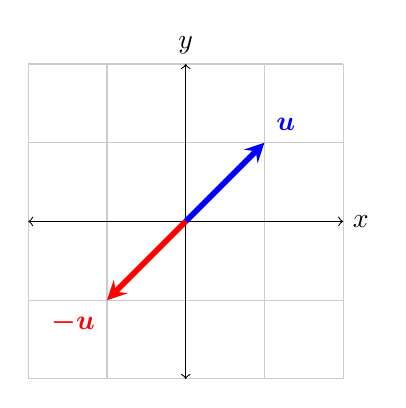
\begin{tikzpicture}
  \draw[thin,gray!40] (-2,-2) grid (2,2);
  \draw[<->] (-2,0)--(2,0) node[right]{$x$};
  \draw[<->] (0,-2)--(0,2) node[above]{$y$};
  \draw[line width=2pt,blue,-stealth](0,0)--(1,1)
        node[anchor=south west]{$\boldsymbol{u}$};
  \draw[line width=2pt,red,-stealth](0,0)--(-1,-1)
        node[anchor=north east]{$\boldsymbol{-u}$};
\end{tikzpicture}
\end{center}
\caption{\label{fig:vectors} Text size inside figure should be as big as
  caption's text. Text size inside figure should be as big as
  caption's text. Text size inside figure should be as big as
  caption's text. Text size inside figure should be as big as
  caption's text. Text size inside figure should be as big as
  caption's text. }
\end{figure}
%% %---------------------------


Here's a typical reference to a floating figure:
Figure~\ref{fig:vectors}. Floats should usually be placed where latex
wants then. Figure\ref{fig:vectors} is centered, and has a caption
that instructs you to make sure that the size of the text within the
figures that you use is as big as (or bigger than) the size of the
text in the caption of the figures. Please do. Really.

In our case, we've explicitly drawn the figure inlined in latex, to
allow this tex file to cleanly compile. But usually, your figures will
reside in some file.pdf, and you'd include them in your document
with, say, \textbackslash{}includegraphics.

Lists are sometimes quite handy. If you want to itemize things, feel
free:

\section{Research Proposal: Search Space Pruning}

\begin{description}
  
\item[fread] a function that reads from a \texttt{stream} into the
  array \texttt{ptr} at most \texttt{nobj} objects of size
  \texttt{size}, returning returns the number of objects read.

\item[Fred] a person's name, e.g., there once was a dude named Fred
  who separated usenix.sty from this file to allow for easy
  inclusion.
\end{description}

\noindent
The noindent at the start of this paragraph in its tex version makes
it clear that it's a continuation of the preceding paragraph, as
opposed to a new paragraph in its own right.


\subsection{LaTeX-ing Your TeX File}
%-----------------------------------

People often use \texttt{pdflatex} these days for creating pdf-s from
tex files via the shell. And \texttt{bibtex}, of course. Works for us.

%-------------------------------------------------------------------------------
\section*{Acknowledgments}
%-------------------------------------------------------------------------------

The USENIX latex style is old and very tired, which is why
there's no \textbackslash{}acks command for you to use when
acknowledging. Sorry.

%-------------------------------------------------------------------------------
\section*{Availability}
%-------------------------------------------------------------------------------

USENIX program committees give extra points to submissions that are
backed by artifacts that are publicly available. If you made your code
or data available, it's worth mentioning this fact in a dedicated
section.

%-------------------------------------------------------------------------------
\bibliographystyle{plain}
\bibliography{\jobname}

%%%%%%%%%%%%%%%%%%%%%%%%%%%%%%%%%%%%%%%%%%%%%%%%%%%%%%%%%%%%%%%%%%%%%%%%%%%%%%%%
\end{document}
%%%%%%%%%%%%%%%%%%%%%%%%%%%%%%%%%%%%%%%%%%%%%%%%%%%%%%%%%%%%%%%%%%%%%%%%%%%%%%%%

%%  LocalWords:  endnotes includegraphics fread ptr nobj noindent
%%  LocalWords:  pdflatex acks
